\section{Taxonomy}
Usually HR tickets can belong to various categories, which can range from a request of shift change to a complaint about a superior. \\
We built a taxonomy of tickets, which is structered in categories and sub categories. Each sub category has its own variables that are used as inputs for the ticket generation. For example to create a request of sick leave, we pass as inputs the reason and the number of days of sick leave requested. Moreover, each category has distinct templates and prompts. The taxonomy has been built following the advise of an HR expert from SAP, however the final taxonomy presented here is a subset of the original one due to the unavailability of public data on certain topics ( Ex. \textit{Work benefits})  \\
The final complete taxonomy can be seen in the \autoref{table:categoriesTable}

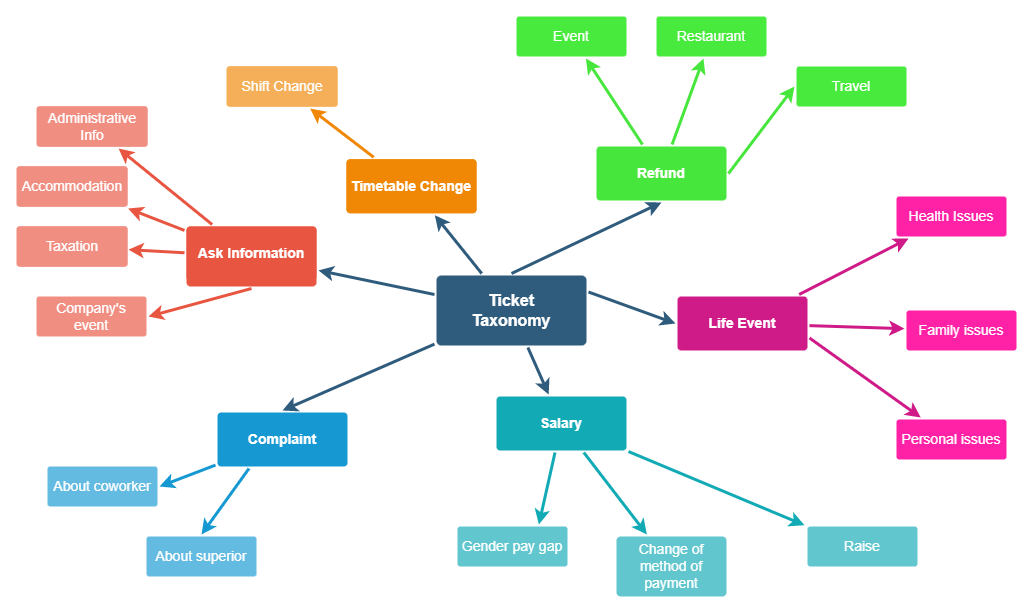
\includegraphics[width=\textwidth]{images/Taxonomy_Tickets.drawio}


\begin{table}[h]
    \resizebox{\textwidth}{!}{
    \begin{tabular}{|l|l|l|}
    \hline
        Category            & Sub-category   & variables                                   \\ \hline
        Ask Information     & Accomodation   & location, duration                          \\
                            & Taxation       & issue                                       \\
        Complaint           & About coworker & complaint                                   \\
                            & About superior & complaint                                   \\
        Timetable change    & Shift change   & reason\_of\_change, old\_date, new\_date    \\
        Salary              & Salary raise   & old\_salary, new\_salary, increase          \\
                            & Gender pay gap & wage\_gap                                   \\
        Life Event          & Health issues  & disease, number\_of\_days\_of\_sick\_leave  \\
                            & Personal issues  & issue, number\_of\_days                   \\
                            & Family issues  & member\_of\_family, issue, number\_of\_days \\
        Refund              & Event          & date, type\_of\_event                       \\
                            & Travel         & from, to, date, vehicle                     \\
                            & Restaurant     & location, date                              \\ \hline
    \end{tabular}
    }
\caption{Table of all defined categories and sub-categories}\label{table:categoriesTable}
\end{table}
    